\documentclass[twocolumn]{aastex631}
\usepackage{graphicx}

\begin{document}

\title{Angular Momentum Alignment Between Stellar Remnants and Dark Matter Halos in Galaxy Mergers}
\author{Ben A Phan}
\date{March 23, 2025}

\begin{abstract}
    This proposal aims to investigate the angular momentum alignment between stellar remnants and their dark matter halos in merged galaxies. In particular, this work focuses on the MW-M31-M33 system simulation. Understanding the stellar structure of galaxies and its relationship with their halos provides insight into the dynamics of dark matter and the evolution of galaxy structures over cosmic time, phenomena that are typically impossible to observe directly. 
\end{abstract}

\section{Introduction}

\subsection{Galaxy-Halo Connection and Angular Momentum}
The angular momentum alignment between stellar structures and their surrounding dark matter halos significantly impacts galaxy formation, structure, and dynamics. According to previous studies (e.g. \cite{Somerville2008, Chua2019, Baptista2023}), galaxy evolution involves complex interactions between baryonic matter and dark matter halos, especially during galaxy mergers when angular momentum is rearranged and realigned.  

\subsection{Significance to Galaxy Evolution}
Understanding the stellar-halo angular momentum connection is crucial, as it strongly affects a galaxy's motion, shape, and star formation rate. Changes in angular momentum alignment can directly alter observable properties such as galaxy size, rotation curves, and stellar velocity dispersion. Investigating these properties provides deeper insight into the stellar-halo relationship, helping to reveal how galaxies interact with their surrounding dark matter environment throughout billions of years of evolution.
 \citep{Chua2019, Baptista2023}.

\subsection{Current Understanding}
Recent studies have significantly improved our understanding on stellar-halo angular momentum alignment. \cite{Somerville2008} demonstrated the importance of realistic dark matter halo models (e.g., NFW profiles and adiabatic contraction) in accurately predicting the weaker observed evolution of galaxies compared to previous prediction model with simpler dark matter profile (see Fig.~\ref{fig:somerville_fig5}). Similarly, \cite{Chua2019} highlighted that stellar and dark matter angular momentum vectors tend to connect more strongly in massive halos at lower redshifts, suggesting this alignment depends on both mass and time. Furthermore, \cite{Baptista2023} showed that evolving stellar-to-halo mass ratios significantly impact the angular momentum distributions, influencing both galaxy formation and evolutionary trajectories.

\begin{figure}[ht!]
    \centering
    \includegraphics[width=0.45\textwidth]{figure5.png}
    \caption{Evolution of average disk sizes normalized to present-day sizes as a function of redshift, with circles representing more detailed halo profiles. The circles show a more gradual size in evolution, which agrees more with observation. This emphasizes predictions from more realistic dark matter halo models. Adapted from \cite{Somerville2008}.}
    \label{fig:somerville_fig5}
\end{figure}

\subsection{Open Questions}
Despite the significant progress on studying this topic, there are still many unknown questions:
\begin{itemize}
    \item How does angular momentum alignment evolve throughout and after galaxy mergers?
    \item What factors govern the strength and persistence of this alignment throughout galaxy evolution?
    \item How does angular momentum realignment affect the structure and kinematics of stellar remnants post-merger?
\end{itemize}

\section{Proposal}

\subsection{Research Question}
This study aims to investigate how angular momentum alignment between stellar remnants and dark matter halos evolves during the MW-M31-M33 merger simulation. Specifically, it seeks to understand the conditions under which alignment strengthens or weakens, and how angular momentum realignment impacts the resulting structure and kinematics of galaxy remnants.

\subsection{Methods}
This analysis will use the provided MW-M31-M33 simulation data, following these specific methods:

\begin{enumerate}
    \item \textbf{Particle Classification and Mass Distribution} (code used from ReadFile, ParticleProperties, and GalaxyMass functions): Identify halo, disk, and bulge particles for each galaxy, then examine their mass and velocity distributions. This will define the evolving mass distribution and structure throughout the merger.
    
    \item \textbf{Center of Mass Analysis} (code used from CenterOfMass and OrbitCOM functions): Calculate the COM positions and velocities for each galaxy at different simulation snapshots, establishing an accurate frame of reference for angular momentum analysis.

    \item \textbf{Angular Momentum Calculation} (code used from Lab 3): Compute the angular momentum vectors of stellar and dark matter halo particles separately. This calculation will use each galaxy’s COM frame, determined by subtracting the galaxy’s COM position and velocity from particle positions and velocities. The angular momentum vectors' magnitudes and directions will be tracked across simulation snapshots, allowing analysis of alignment evolution throughout the merger process.

    \item \textbf{Galaxy Morphology and Shape Evolution} (code used from Lab 6 and Lab 7): Apply contour plots to quantify changes in halo and stellar morphology, demonstrating the impact of mergers on the shape of the galaxy and its halo.
\end{enumerate}


To demonstrate my approach, I will include a visualization of angular momentum alignment over time. The following figure presents the evolution of angular momentum alignment for the MW's stellar and halo components, plotted against  time:

\begin{figure}[ht!]
    \centering
    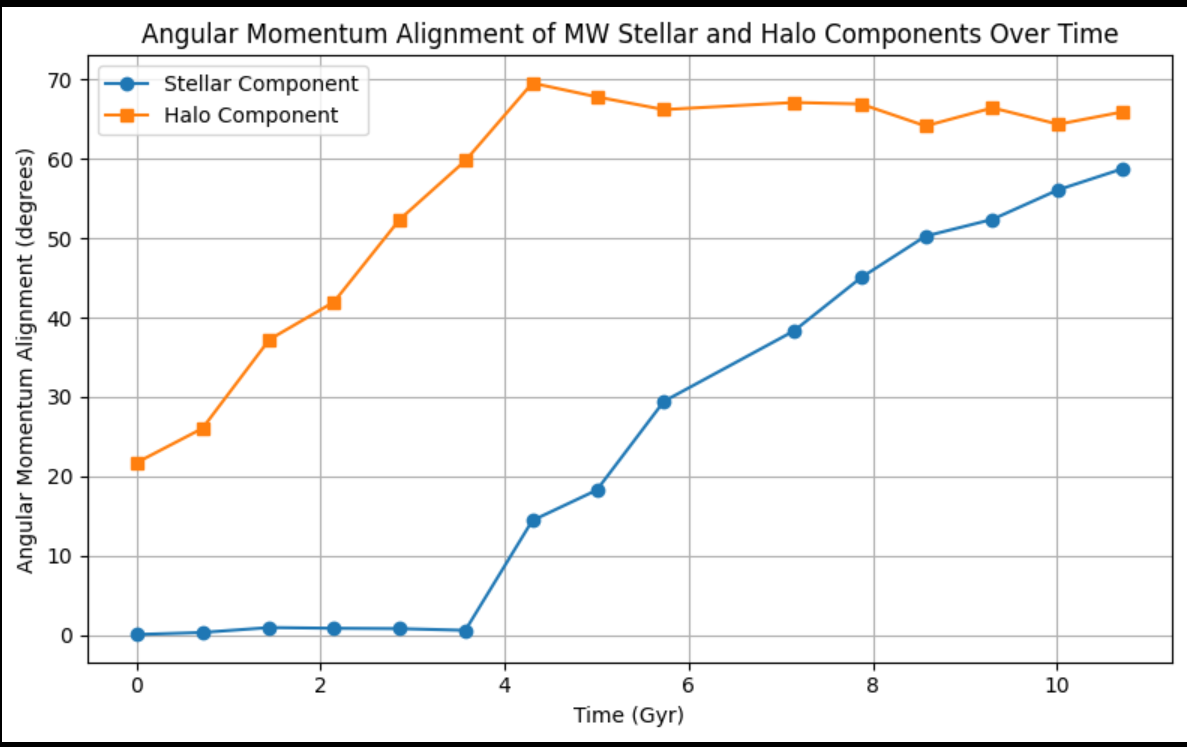
\includegraphics[width=0.45\textwidth]{MW_Angular_Momentum_Alignment_Time.png}
    \caption{Evolution of angular momentum alignment for MW's stellar and halo components over time. The y-axis represents the alignment angle in degrees, while the x-axis represents time in Gyr. This visualization demonstrates how the angular momentum of the stellar and halo components evolves throughout the merger.}
    \label{fig:angular_momentum_alignment}
\end{figure}


\subsection{Hypothesis}
I hypothesize that:
\begin{itemize}
    \item Initially, stellar and halo angular momentum vectors have minimal alignment as they have separate formation histories.
    \item During the merger, gravity from merging galaxies and their tidal forces will significantly rearrange angular momentum, increasing the alignment between stellar and halo components.
    \item Post-merger, stellar remnants will show stronger and more rapid angular momentum alignment than dark matter halos due to their more centralized mass distribution and collisional interactions.
\end{itemize}


\bibliography{cite.bib}
\bibliographystyle{aasjournal}

\end{document}